\documentclass[]{paper}
\usepackage{amsmath}
\usepackage{amssymb}
\usepackage{float}
\usepackage{algorithm}
\usepackage{algpseudocode}
\usepackage{tikz}
\usetikzlibrary{positioning,arrows.meta}

\newcommand{\keep}{\textsc{keep}}
\newcommand{\edit}{\textsc{edit}}
\newcommand{\drop}{\textsc{drop}}
\newcommand{\add}{\textsc{add}}
\newcommand{\pend}[1]{\textbf{[#1]}}

\definecolor{done}{HTML}{B7DEC3}
\definecolor{partial}{HTML}{F3DFA2}
\definecolor{missing}{HTML}{D7DADF}

\begin{document}

\title{DiffusEdit: Progress Report}

\author[*]{Tatva Agarwal}
\author[*]{Vedant Kulkarni}
\author[*]{Byasani Vedavyas}
\author[*]{Venya Velmurugan}

\affiliation[]{IIIT Hyderabad}

\contribution[*]{Equal contribution; authors listed alphabetically.}

\abstract{
This report describes how the DiffusEdit training data was built and the first experiments run on it, on one A100 GPU\@. The data comes from FRUIT-Wiki. A greedy sentence aligner labels each source sentence \keep{}, \edit{}, or \drop{}, and a word-level diff marks the stale tokens of each \edit{} sentence. A confident-learning estimate puts the label error rate at 39 to 59\% per class, but a hand review of the 111 sentences that estimate disputes most found 21.6\% wrong, so the estimate overstates the noise. On frozen LLaDA-8B hidden states, a linear sentence classifier reaches macro-F1 0.499, against 0.433 for a baseline without LLaDA, and neither focal loss nor any evidence feature raises it. The token staleness head ranks stale tokens only slightly above correct ones (AUROC 0.645), and no threshold on its scores reaches precision above 0.573. When infilling uses the true stale tokens as masks, the frozen model writes 21.8\% of the entities the update adds and uses the evidence to do so. With the staleness head's masks, the output scores below the unchanged sentence on ROUGE-L, entity precision and entity recall, at Holm-corrected $p \le 0.003$. Every number comes from training articles held out from training. The validation and test splits were not used.
}

\date{October 3, 2026}
\correspondence{\email{vedant.kulkarni@students.iiit.ac.in}}

\maketitle{}

\section{Introduction}
\label{sec:intro}

The design document describes DiffusEdit as a loop of four stages built on a frozen masked diffusion model \citep{nie-etal-2025-llada, zou-etal-2026-detect}. A sentence classifier labels each article sentence \keep{}, \edit{}, or \drop{}. A token staleness head chooses which tokens of an \edit{} sentence to mask. The frozen model infills the masks at four replacement lengths and keeps the best-scoring candidate. A cascade detector then flags sentences that the repairs made wrong, and the loop repeats.

This report covers the data the heads train on and the first three stages, run once. It answers four questions.

\begin{enumerate}
\item How were the training labels made, and how many of them are wrong?
\item How well do small heads on frozen LLaDA hidden states find the sentences and the tokens that need to change?
\item Given correct masks, does the frozen model write the new facts from the evidence into the masked positions?
\item How much of the gap between correct and predicted masks comes from the staleness head?
\end{enumerate}

\Cref{sec:background} explains the measurements. \Cref{sec:data} describes how the data was built, how the aligner works, and what the label audit found. \Cref{sec:setup} covers the hardware and the state of the pipeline. \Cref{sec:classifier,sec:staleness,sec:infilling} report the three components, and \Cref{sec:tests} tests which differences survive a correction for multiple comparisons. \Cref{sec:examples} shows examples of each problem from the data and the runs, \Cref{sec:findings} lists the findings and the next steps, and \Cref{app:code} documents the code and its algorithms.

\section{Background}
\label{sec:background}

\subsection{Held-Out Data}

A model fitted on some data scores better on that data than on new data. To measure how a head behaves on articles it has not seen, we set aside a fixed 10\% of the training articles before training and call this part the \emph{held-out} set. It plays the role the validation set plays in the design document. The validation and test splits stay untouched for later work.

\subsection{Classification Measures}

For one class, \emph{precision} is the share of items predicted as that class that belong to it, and \emph{recall} is the share of the class's items that the model predicted. The \emph{F1 score} is their harmonic mean. \emph{Macro-F1} averages the F1 of the three sentence classes, so the frequent \keep{} class does not dominate the average.

A head that outputs a score per item can trade precision against recall by moving its threshold. The \emph{AUROC} is the probability that a random positive item scores higher than a random negative one. A random scorer has AUROC 0.5 and a perfect one 1.0. \emph{PR-AUC} is the area under the curve of precision against recall.

\subsection{Infilling Measures}

Each repaired sentence has a \emph{gold rewrite}, the corrected sentence from the later Wikipedia version. We compare the system's output with it.

\emph{ROUGE} \citep{lin-2004-rouge} counts shared word sequences between two texts. ROUGE-1 counts single words, ROUGE-2 word pairs, and ROUGE-L the longest common subsequence, each as an F1 score. In a repaired sentence most words did not change, so sentence-level ROUGE-L mostly measures how much of the unchanged text survives. \emph{UpdateROUGE} \citep{iv-etal-2022-fruit} restricts ROUGE to the sentences an update touched. For one article it compares the output sentences that do not appear verbatim in the source article with the gold sentences that do not appear verbatim in the source.

\emph{Entity measures} follow Section~9.2 of the design document. A mention extractor $M$ returns the named entities of 13 types found by the spaCy model \texttt{en\_core\_web\_sm} 3.8.0, lowercased, together with every digit string. It is the extractor that produced the mentions stored in the data. With $G$, $S$, $O$ and $E$ the mentions of the gold rewrite, the source sentence, the output and the article's evidence,
\begin{align*}
\text{precision} &= \frac{|O \cap G|}{|O|}, &
\text{recall} &= \frac{|O \cap G|}{|G|}, &
\text{new-entity recall} &= \frac{|O \cap (G \setminus S)|}{|G \setminus S|}, \\
\text{outdated kept} &= \frac{|O \cap (S \setminus G)|}{|S \setminus G|}, &
\text{fabricated} &= \frac{|O \setminus (S \cup E)|}{|O|}.
\end{align*}
New-entity recall measures the facts the update adds. Outdated kept measures the facts the update removes but the output still contains, and fabricated counts entities found in neither the source nor the evidence. Lower is better for the last two. Each measure sums numerators and denominators over all repaired sentences before dividing.

\subsection{Significance Tests}

A difference between two systems measured on 50 articles can arise by chance. We test each difference with two procedures that treat the article as the unit, because sentences of one article are not independent. The \emph{paired bootstrap} \citep{efron-tibshirani-1993-bootstrap} draws 50 articles with replacement, recomputes the difference, and repeats 10,000 times, and the middle 95\% of the recomputed differences is the 95\% confidence interval. The \emph{paired permutation test} swaps the outputs of the two systems inside each article with probability one half and repeats 10,000 times. The $p$-value is the share of permuted differences at least as large in magnitude as the observed one.

Running 30 tests at the 0.05 level produces about 1.5 false positives even when no true difference exists. The \emph{Holm correction} \citep{holm-1979-simple} raises each $p$-value so that the chance of any false positive across a table of tests stays at or below 0.05. We call a difference significant when its Holm-corrected $p$ is below 0.05.

\section{Data}
\label{sec:data}

\subsection{Source}

FRUIT-Wiki \citep{iv-etal-2022-fruit} pairs the introduction of an English Wikipedia article in one yearly snapshot with the same introduction a year later, together with evidence snippets taken from other Wikipedia articles. The training shards cover November 2019 to November 2020, and the gold test set, which annotators checked, covers November 2020 to November 2021. The FRUIT authors publish the data as TFRecord files in their EdiT5 format. Our loader, \texttt{datasets/fruit/load.py}, reads them in pure Python without TensorFlow.

Each record has an input string and a target string. The input lists the source sentences behind markers \texttt{[0]}, \texttt{[1]}, \ldots, then the marker \texttt{[CONTEXT]}, then the evidence snippets behind markers \texttt{(0)}, \texttt{(1)}, \ldots. The target is a sequence of operations. A marker \texttt{[i]} copies source sentence $i$ unchanged. Any other text is a generated span, a new or rewritten passage, and the evidence markers in front of it name the snippets it cites. A source sentence whose marker is missing from the target was deleted or rewritten. Splitting each generated span into sentences with spaCy gives the target sentences. In the training data, 158,318 target sentences are copies and 311,051 are generated.

\subsection{Build}

\texttt{datasets/collate.py} turns each FRUIT instance into one record in five steps.

\begin{enumerate}
\item Parse the record into source sentences, target sentences and evidence.
\item Drop the instance if the source article exceeds 400 LLaDA tokens.
\item Align source and target sentences and label every source sentence (\Cref{sec:aligner}).
\item Drop the instance if no source sentence is \edit{} or \drop{}, because an update that only adds sentences needs an insertion step the design does not have.
\item Extract mentions, classify each change as direct or candidate for cascade mining, and cut the evidence to 600 tokens (\Cref{sec:evidence}).
\end{enumerate}

\Cref{fig:data_build}(a) shows what the filters remove. Of 102,902 training instances, 8,515 have articles over the budget and 16,955 only add sentences, which leaves 77,432. The dev shard keeps 8,685 of 11,561. A seeded draw (seed 20260927) takes 2,000 of the dev records as the validation split, and the other 6,685 join training, so the training split has 84,117 articles. The gold test set keeps 730 of its 914 instances.

\begin{figure}[t]
\centering
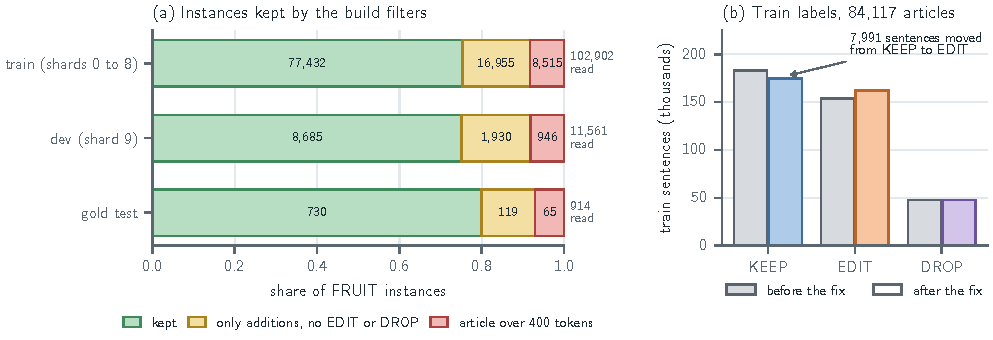
\includegraphics[width=\linewidth]{figures/data_build.pdf}
\caption{Data build. (a)~FRUIT instances per source and the filter that removed them. The dev shard supplies the 2,000-article validation split, and its other kept instances join training. (b)~Labels of the 384,788 training source sentences before and after the \keep{} fix (\Cref{sec:keepfix}).}
\label{fig:data_build}
\end{figure}

\subsection{The Sentence Aligner}
\label{sec:aligner}

The target article does not say which target sentence a rewritten source sentence became, so the aligner infers it from word overlap. It lowercases each sentence and splits it into word tokens and single punctuation marks. The \emph{similarity} of a source sentence $s$ and a target sentence $t$ is the F1 overlap of their token multisets. With $c$ the number of tokens they share, counting repeats,
\[
\text{sim}(s, t) = \frac{2 \cdot \frac{c}{|s|} \cdot \frac{c}{|t|}}{\frac{c}{|s|} + \frac{c}{|t|}}.
\]
The aligner scores every source-target pair and sorts the pairs by similarity, breaking ties by the distance between the two sentence positions and then by source position. It walks down the list and accepts a pair when neither sentence is taken yet, stopping when the similarity falls below 0.35. Each sentence takes part in at most one pair. The labels follow from the pairs.

\begin{itemize}
\item A source sentence without a partner is \drop{}.
\item A source sentence with similarity at least 0.95 to its partner, and no changed word that contains a capital letter or a digit, is \keep{}.
\item Every other paired source sentence is \edit{}.
\item A target sentence without a partner is an addition (\add{}). Additions get no label, because the design does not insert sentences.
\end{itemize}

\Cref{tab:align_example} shows one training article. The first source sentence is closer to the second target sentence (0.80) than to the first (0.44), so the aligner pairs it with the second, and the first target sentence becomes an addition. The third source sentence reaches at most 0.29 against any target sentence and becomes \drop{}. Algorithm~\ref{alg:align} in \Cref{app:code} gives the procedure.

\begin{table}[t]
\caption{Alignment of training article \texttt{train-002320}. Similarity is the token-multiset F1 with each target sentence. Bold marks the accepted pair. The stale spans of the \edit{} sentence are underlined.}
\label{tab:align_example}
\centering
\footnotesize
\begin{tabular}{p{0.44\linewidth}ccc l}
\toprule
Source sentence & T0 & T1 & T2 & Label \\
\midrule
S0: \underline{The Appian Way Regional Park} is a protected area of around \underline{3400} hectares, established by the Italian region of Latium. & 0.44 & \textbf{0.80} & 0.23 & \edit{} $\to$ T1 \\
S1: It falls primarily within the territory of Rome but parts also extend into the neighbouring towns of Ciampino and Marino. & 0.18 & 0.26 & \textbf{1.00} & \keep{} $\to$ T2 \\
S2: The Catacombs of Rome and Colli Albani (Rome Metro) are nearby. & 0.16 & 0.19 & 0.29 & \drop{} \\
\midrule
\multicolumn{5}{p{0.95\linewidth}}{T0 (\add{}): The Appian Way Regional Park is the second-largest urban park of Europe, after Losiny Ostrov National Park in Moscow.} \\
\multicolumn{5}{p{0.95\linewidth}}{T1: It is a protected area of around 4580 hectares, established by the Italian region of Latium.} \\
\multicolumn{5}{p{0.95\linewidth}}{T2: copy of S1.} \\
\bottomrule
\end{tabular}
\end{table}

\Cref{fig:aligner} shows the best-match similarity of the source sentences of 10,000 random training articles. Most \keep{} sentences sit at 1.0, \edit{} sentences spread between 0.35 and 1.0, and \drop{} sentences sit mostly below 0.35. Two groups cross the cut-offs. 1,358 \drop{} sentences have a partner above 0.35 that another source sentence took first. 1,002 \edit{} sentences reach 0.95 or more but changed a name or a number.

\begin{figure}[t]
\centering
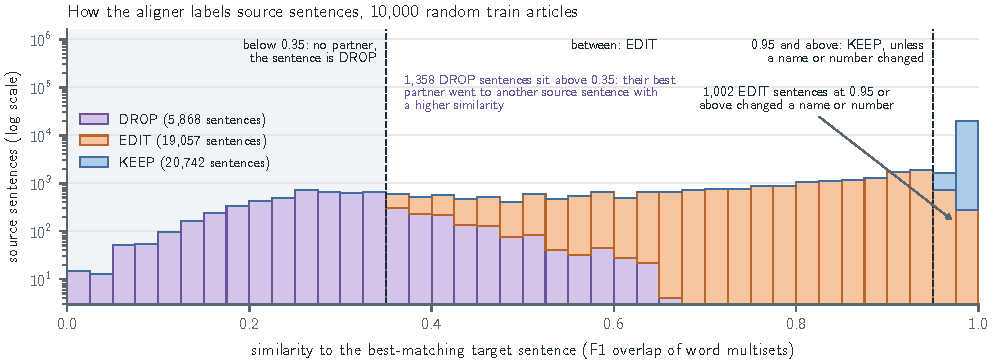
\includegraphics[width=\linewidth]{figures/aligner.pdf}
\caption{Similarity of each source sentence to its best-matching target sentence, stacked by the final label, for the 45,667 source sentences of 10,000 random training articles. The y axis is logarithmic. Dashed lines mark the two cut-offs of the aligner.}
\label{fig:aligner}
\end{figure}

\subsection{Token Labels}

For each \edit{} sentence, a word-level diff marks which tokens changed. The diff is Python's \texttt{difflib} sequence matcher over the lowercased tokens of the source sentence and its partner, which finds the longest matching blocks and reports the rest as replaced, deleted or inserted. Replaced and deleted source tokens are \emph{stale}. An insertion has no source token, so the token just before it becomes stale, which lets a mask at that position grow into the inserted text. Adjacent stale tokens merge into character spans. In \Cref{tab:align_example}, the diff marks \emph{The Appian Way Regional Park} (rewritten as \emph{It}) and \emph{3400} (rewritten as \emph{4580}). The first change is stylistic. The evidence does not prompt it, but the label still marks it stale.

\subsection{The KEEP Fix}
\label{sec:keepfix}

The first build labelled a pair \keep{} on similarity alone. A long sentence whose only change is a new club name or a new year keeps a similarity above 0.95, so these updates were labelled \keep{}. The fix adds the second condition of \Cref{sec:aligner}, that no changed word contains a capital letter or a digit. Applied to the existing records, it moved 7,991 training sentences from \keep{} to \edit{} and changed nothing else (\Cref{fig:data_build}(b)). The training split now holds 174,873 \keep{}, 162,053 \edit{} and 47,862 \drop{} sentences.

\subsection{Evidence Budget}
\label{sec:evidence}

The evidence of one article may hold at most 600 LLaDA tokens. The build orders the snippets by how many mentions they share with the article, most first, and adds them whole while the budget allows. The first snippet that does not fit is cut, by binary search over its token count, to the longest prefix that fits. Every snippet after it is left empty. In the training split, 45.6\% of articles lose evidence this way, and 14.9\% of the 516,999 snippets end up empty.

\subsection{Label Noise}
\label{sec:noise}

The labels are \emph{silver}. The aligner made them automatically, and no person checked them. Two measurements of their error rate exist, and they disagree.

\paragraph{Confident learning.} \emph{Confident learning} \citep{northcutt-etal-2021-confident} estimates label errors from a classifier's held-out predictions. A sentence classifier was trained in folds on the LLaDA features of an earlier 20,000-article extraction, so that every sentence received probabilities from a model that had not trained on it. The out-of-fold macro-F1 was 0.506. For each class, the method sets a threshold equal to the mean probability the model gives that class on sentences labelled with it (0.448 for \keep{}, 0.491 for \edit{}, 0.348 for \drop{}). A sentence counts toward the class with the highest probability among those above their thresholds, and the counts, rescaled to the label totals, form the \emph{confident joint} of \Cref{fig:label_noise}(a). Off-diagonal cells are estimated errors. The estimate is 39.8\% of \keep{}, 39.3\% of \edit{} and 59.0\% of \drop{} labels wrong, 42.0\% of 91,699 sentences overall. These are the figures the earlier documents quote as 40 to 60\%. The labels predate the fix of \Cref{sec:keepfix}, and the script that produced them, \texttt{classifier/noise.py}, is not in the repository. Only its output, \texttt{audit/noise.json}, is.

\paragraph{Hand review.} The confident-learning estimate cannot separate a wrong label from a classifier mistake, and this classifier scores macro-F1 0.506, so many disputed sentences may be classifier errors. The audit sheet \texttt{audit/flagged.tsv} holds the 300 sentences the classifier disputes most confidently. One reviewer has judged 117 of them, 6 of which were bad sentence splits. Of the other 111, 24 labels were wrong, 21.6\% with a 95\% Wilson interval of 15.0 to 30.2\%. By given label, 8 of 65 \keep{} (12.3\%), 13 of 33 \edit{} (39.4\%) and 3 of 13 \drop{} (23.1\%) were wrong. \Cref{fig:label_noise}(b) compares these rates with the estimate.

\paragraph{Conclusion.} The flagged sentences are the ones most likely to be wrong, yet only 21.6\% of them are. The confident-learning figure of 40 to 60\% therefore overstates the label noise, and the earlier documents should not quote it as measured. The noise rate of a random sample is unknown. The sheet \texttt{audit/train\_audit.tsv}, every sentence of 100 random training articles (436 sentences), exists for that measurement, but nobody has reviewed it yet. The review above also predates the \keep{} fix. Eight of its 24 errors are \keep{} labels that should be \edit{}, the kind of error the fix targets.

\begin{figure}[t]
\centering
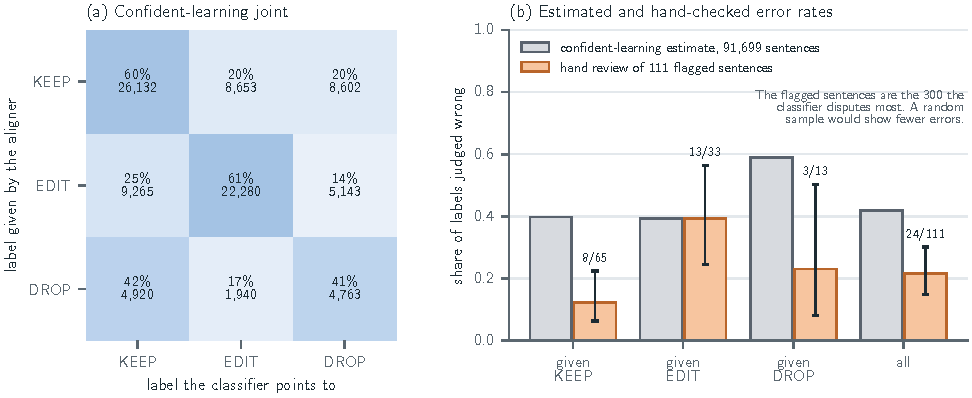
\includegraphics[width=\linewidth]{figures/label_noise.pdf}
\caption{Label noise. (a)~Confident joint of 91,699 sentences: the label the aligner gave against the label the classifier's probabilities point to, as a share of each row and as a count. Off-diagonal cells count as estimated errors. (b)~The confident-learning error estimate per given label, and the share of wrong labels a reviewer found among the 111 judged flagged sentences, with 95\% Wilson intervals and counts.}
\label{fig:label_noise}
\end{figure}

\subsection{Held-Out Split and Supported Sentences}

The held-out set has 8,256 articles, 38,267 sentences, and 531,706 tokens inside \edit{} sentences. A seeded draw over article indices chooses it (seed 42 unless stated otherwise), and all heads hold out the same articles for one seed.

We call an \edit{} sentence \emph{supported} when every word of its gold rewrite that is missing from the source sentence appears in the source or in the article's evidence. Only for supported sentences does the input hold every new fact. In the first infilling run, 57 of the 338 sentences whose rewrite adds words were supported (16.9\%). The held-out set contains 2,557 supported sentences in 2,280 articles.

\section{Setup}
\label{sec:setup}

All GPU work ran on one NVIDIA A100 with 40~GB of memory. The model is LLaDA-8B-Base \citep{nie-etal-2025-llada} at revision \texttt{0f2787f}, in bf16 without quantization. One forward pass per article reads the evidence followed by the article and stores the mean hidden state of each source sentence and of each evidence snippet at blocks 24 and 32 of 32, and the block-32 state of every token inside an \edit{} sentence. The pass took 1~hour 40~minutes for 84,117 articles and produced no non-finite values. The stored features occupy about 55~GB.

\Cref{fig:pipeline} shows which parts of the design exist. The cascade detectors, the consequence head and the loop over rounds are not built. The infilling runs therefore run one round, and they take the sentence labels from the data rather than from the classifier.

\begin{figure}[t]
\centering
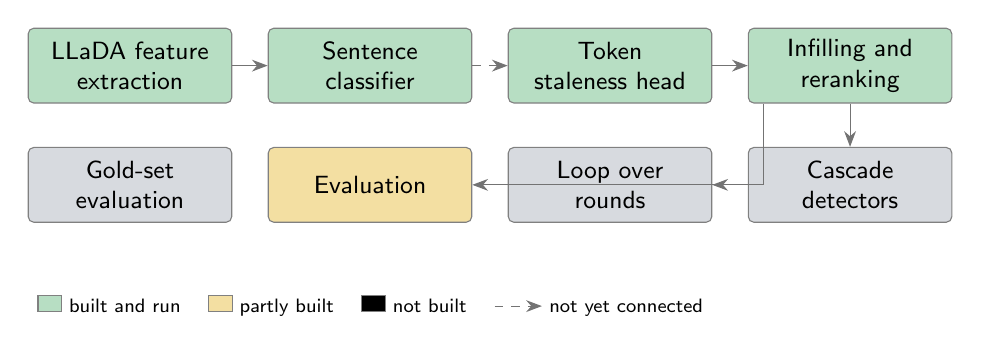
\begin{tikzpicture}[
  box/.style={draw=black!50, rounded corners=2pt, minimum height=0.95cm, text width=2.35cm, align=center, font=\small\sffamily},
  arr/.style={-{Stealth[length=2mm]}, black!55}]
\node[box, fill=done] (ext) {LLaDA feature\\extraction};
\node[box, fill=done, right=0.45cm of ext] (cls) {Sentence\\classifier};
\node[box, fill=done, right=0.45cm of cls] (sta) {Token\\staleness head};
\node[box, fill=done, right=0.45cm of sta] (inf) {Infilling and\\reranking};
\node[box, fill=missing, below=0.55cm of inf] (cas) {Cascade\\detectors};
\node[box, fill=missing, left=0.45cm of cas] (loop) {Loop over\\rounds};
\node[box, fill=partial, left=0.45cm of loop] (ev) {Evaluation};
\node[box, fill=missing, left=0.45cm of ev] (gold) {Gold-set\\evaluation};
\draw[arr] (ext) -- (cls);
\draw[arr, dashed] (cls) -- (sta);
\draw[arr] (sta) -- (inf);
\draw[arr] (inf) -- (cas);
\draw[arr] (cas) -- (loop);
\draw[arr] (inf.south west) ++(0.2,0) |- (ev.east);
\node[font=\scriptsize\sffamily, anchor=west] at ([yshift=-1.05cm]gold.south west) {%
\tikz\fill[done, draw=black!50] (0,0) rectangle (0.3,0.2); built and run \quad
\tikz\fill[partial, draw=black!50] (0,0) rectangle (0.3,0.2); partly built \quad
\tikz\fill[missing, draw=black!50] (0,0) rectangle (0.3,0.2); not built \quad
\tikz\draw[arr, dashed] (0,0.1) -- (0.6,0.1); not yet connected};
\end{tikzpicture}
\caption{Pipeline components and their current state. Infilling reads the derived sentence labels, not the classifier output. Evaluation covers ROUGE, UpdateROUGE, entity measures and significance tests, but not AlignScore, edit distance, or the gold set.}
\label{fig:pipeline}
\end{figure}

\section{Sentence Classifier}
\label{sec:classifier}

\subsection{Method}

The classifier is one linear layer that maps the mean hidden state of a sentence to three scores, followed by a softmax (Eq.~5 of the design document). Inputs are standardized with the mean and standard deviation of the training part. The default loss is cross-entropy with class weights $w_c = N / (3 N_c)$, where $N_c$ counts the training sentences of class $c$, which raises the cost of mistakes on the rare \drop{} class. Training uses AdamW with learning rate $10^{-3}$, weight decay $10^{-2}$ and batches of 1024 sentences, and stops after 3 epochs without a gain in held-out macro-F1. A sentence is deleted only when its \drop{} probability reaches a gate $\tau_d$, tuned on the held-out set between 0.35 and 0.95. A sentence that favors \drop{} below the gate becomes \edit{}.

\emph{Focal loss} \citep{lin-etal-2017-focal} multiplies the loss of each sentence by $(1 - p_y)^\gamma$, where $p_y$ is the probability the head gives the true label. With the class weights kept,
\[
\mathcal{L}_{\text{focal}} = -\sum_j w_{y_j} (1 - p_{j, y_j})^{\gamma} \log p_{j, y_j}.
\]
With $\gamma = 0$ it is the weighted cross-entropy. With $\gamma = 2$, the value we use, a sentence the head already gets right with probability 0.9 contributes one hundredth of its cross-entropy loss, so training concentrates on hard sentences.

The baseline embeds each sentence and each evidence snippet with the sentence encoder all-MiniLM-L6-v2 \citep{wang-etal-2020-minilm, reimers-gurevych-2019-sentence}, which never sees the evidence and the sentence together, and trains the same head on the sentence vector joined to the mean snippet vector. The evidence ablation joins one evidence vector to each LLaDA sentence vector. The vector is the mean of the article's snippet vectors, the snippet with the highest cosine similarity to the sentence, or an attention-weighted sum whose weights come from learned projections of the sentence and snippet vectors.

Every configuration ran with five seeds, 42, 1, 2, 3 and 4. A seed fixes the held-out split, the initialization and the batch order, so the spread across seeds measures how much a result depends on these choices.

\subsection{Results}

\Cref{tab:classifier} and \Cref{fig:classifier,fig:seeds} report the held-out results. LLaDA at block 24 reaches macro-F1 0.499 with seed 42, 0.066 above the baseline. Across five seeds the mean is 0.499 with standard deviation 0.002, against 0.436 with standard deviation 0.003 for the baseline. The rerun with seed 42 reproduced the original 0.4993 exactly. Block 24, at three quarters of the depth, scores 0.009 above the final block on average. \drop{} is the weakest class, with precision 0.240, so about three of every four predicted deletions are wrong.

Focal loss lowers macro-F1 at both blocks, to 0.490 at block 24 and 0.480 at block 32, means over five seeds. No evidence input raises macro-F1 either. The mean, nearest and attention variants score between 0.004 and 0.016 below the sentence vector alone. The attention weights collapse onto a single snippet, with a mean largest weight of 0.999.

\Cref{tab:classifier_tests} tests these differences. With seed 42, every model of the comparison holds out the same 38,267 sentences, so the paired bootstrap and permutation test of \Cref{sec:background} apply, with the article as the unit and 2,000 resamples. Each resample recomputes macro-F1, with each model's own \drop{} gate. All four differences are significant after the Holm correction, and on each of the five seeds the difference has the same sign.

\begin{table}[t]
\caption{Paired tests between sentence classifiers. The interval and $p$-values come from seed 42 (38,267 held-out sentences in 8,256 articles, 2,000 resamples, so the smallest attainable $p$ is 0.0005). The last column gives the difference on each seed's own held-out split, as mean $\pm$ standard deviation over five seeds.}
\label{tab:classifier_tests}
\centering
\footnotesize
\begin{tabular}{lccccc}
\toprule
Comparison (A $-$ B) & Macro-F1 A $-$ B & 95\% interval & $p$ & $p_{\text{Holm}}$ & 5 seeds \\
\midrule
Block 24 $-$ MiniLM baseline & $+0.067$ & $[+0.059, +0.074]$ & $<0.001$ & \textbf{0.002} & $+0.064 \pm 0.002$ \\
Block 24 $-$ block 32 & $+0.009$ & $[+0.003, +0.016]$ & 0.006 & \textbf{0.006} & $+0.009 \pm 0.002$ \\
Block 24 cross-entropy $-$ focal & $+0.010$ & $[+0.006, +0.013]$ & $<0.001$ & \textbf{0.002} & $+0.010 \pm 0.002$ \\
Block 32 cross-entropy $-$ focal & $+0.013$ & $[+0.006, +0.019]$ & $<0.001$ & \textbf{0.002} & $+0.009 \pm 0.003$ \\
\bottomrule
\end{tabular}
\end{table}

\begin{table}[t]
\caption{Sentence classifier on 38,267 held-out sentences with seed 42 (17,652 \keep{}, 16,100 \edit{}, 4,515 \drop{}), and the mean and standard deviation of macro-F1 over five seeds. $\tau_d$ is the tuned deletion gate of the seed-42 run.}
\label{tab:classifier}
\centering
\footnotesize
\setlength{\tabcolsep}{4pt}
\begin{tabular}{lcccccc}
\toprule
Model & Macro-F1 & \keep{} F1 & \edit{} F1 & \drop{} F1 & $\tau_d$ & 5 seeds \\
\midrule
MiniLM baseline & 0.433 & 0.440 & 0.580 & 0.278 & 0.40 & $0.436 \pm 0.003$ \\
LLaDA block 24, cross-entropy & \textbf{0.499} & 0.558 & 0.626 & 0.315 & 0.45 & $\mathbf{0.499 \pm 0.002}$ \\
LLaDA block 32, cross-entropy & 0.490 & 0.534 & 0.611 & 0.327 & 0.45 & $0.490 \pm 0.002$ \\
LLaDA block 24, focal & 0.490 & 0.549 & 0.608 & 0.312 & 0.35 & $0.490 \pm 0.002$ \\
LLaDA block 32, focal & 0.478 & 0.534 & 0.603 & 0.298 & 0.40 & $0.480 \pm 0.002$ \\
\midrule
\multicolumn{7}{l}{Block 24 with an evidence vector: mean 0.495, nearest 0.486, attention 0.488} \\
\multicolumn{7}{l}{Block 32 with an evidence vector: mean 0.486, nearest 0.474, attention 0.481} \\
\bottomrule
\end{tabular}
\end{table}

\begin{figure}[t]
\centering
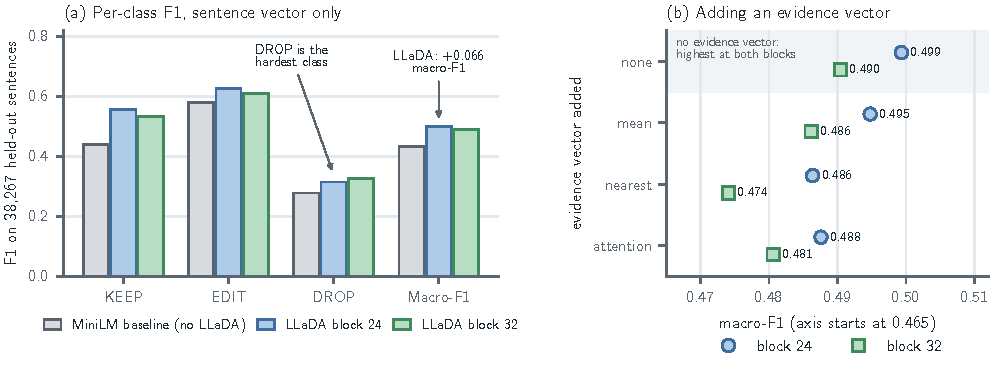
\includegraphics[width=\linewidth]{figures/classifier.pdf}
\caption{Sentence classifier on the held-out set, seed 42. (a)~Per-class F1 and macro-F1 of the baseline and of LLaDA at blocks 24 and 32, using the sentence vector alone. (b)~Macro-F1 when an evidence vector joins the LLaDA sentence vector. The x axis of panel (b) starts at 0.465.}
\label{fig:classifier}
\end{figure}

\begin{figure}[t]
\centering
\IfFileExists{figures/seeds.pdf}{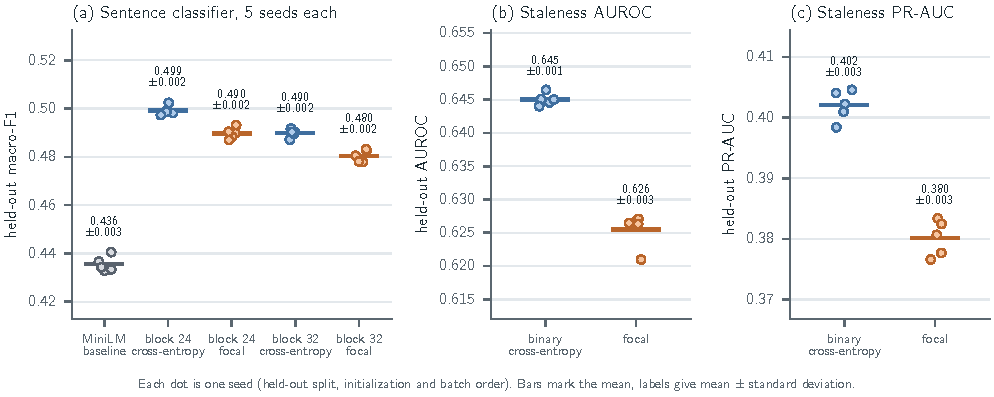
\includegraphics[width=\linewidth]{figures/seeds.pdf}}{\fbox{\parbox{0.9\linewidth}{\centering\sffamily Figure pending: the seed and focal-loss runs are still on the instance.}}}
\caption{Five seeds per configuration. (a)~Held-out macro-F1 of the sentence classifier. (b) and (c)~Held-out AUROC and PR-AUC of the staleness head. Each seed draws its own held-out split, so the spread includes the effect of which articles are held out.}
\label{fig:seeds}
\end{figure}

\section{Token Staleness Head}
\label{sec:staleness}

\subsection{Method}

The staleness head is one linear layer with a sigmoid on the block-32 state of each token inside an \edit{} sentence (Eq.~7 of the design document). Its output, the \emph{staleness score}, lies between 0 and 1. The head trains on 4,804,230 tokens, 28.2\% of them stale, with binary cross-entropy and a weight of 2.54 on stale tokens. The threshold $\tau$ that maximizes token F1 on the held-out set is 0.40, and a token with score at least $\tau$ is masked. The focal variant uses the binary form of the focal loss with $\gamma = 2$ and the same weight on stale tokens.

\subsection{Results}

On 531,706 held-out tokens, 28.5\% of them stale, the head reaches AUROC 0.645 and PR-AUC 0.405 with seed 42. Over five seeds, binary cross-entropy gives AUROC $0.645 \pm 0.001$ and PR-AUC $0.402 \pm 0.003$. Focal loss lowers both, to AUROC $0.626 \pm 0.003$ and PR-AUC $0.380 \pm 0.003$ (\Cref{fig:seeds}). The five seeds of the two losses do not overlap on either measure.

\Cref{fig:stale_scores}(a) shows why the AUROC is low. Stale and correct tokens have almost the same score distribution. \Cref{fig:stale_scores}(b) groups tokens by score and plots the share that is stale in each group. The share rises steadily from 0.06 at scores near 0.1 to 0.62 at scores near 0.9, so the scores order tokens in the right direction. The share passes one half only above a score of 0.81, where 2.1\% of tokens lie. Among tokens scored near 0.6, only 35\% are stale, because the weight of 2.54 on stale tokens shifts every score upward.

\begin{figure}[t]
\centering
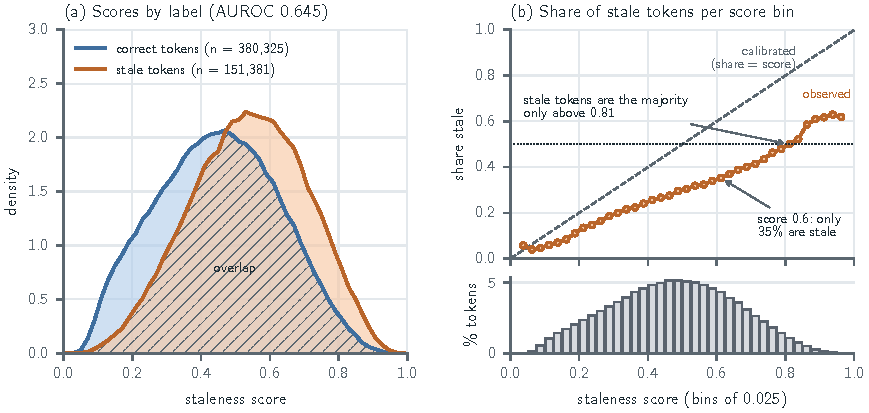
\includegraphics[width=\linewidth]{figures/stale_scores.pdf}
\caption{Staleness scores on 531,706 held-out tokens, seed 42. (a)~Density of the score for stale and correct tokens. The hatched area is where the two densities overlap. (b)~Share of stale tokens among tokens in each score bin of width 0.025, with bins of fewer than 50 tokens omitted. A calibrated score would follow the dashed diagonal. The lower panel shows the share of all tokens in each bin.}
\label{fig:stale_scores}
\end{figure}

\subsection{Threshold Rules}

\Cref{tab:rules} and \Cref{fig:stale_rules} compare five rules for choosing which tokens to mask. Each row reports precision (the share of masked tokens that are stale), recall (the share of stale tokens that are masked), and the share of all tokens masked.

The tuned threshold $\tau = 0.40$ masks 65.3\% of tokens, and about two of every three masked tokens were correct. Raising $\tau$ to 0.60 matches the masked share to the stale share and raises precision to 0.415, but then 62\% of stale tokens stay unmasked. Masking the top 28.5\% of each sentence gives the same trade as a global threshold.

The last row is an upper bound. Any threshold rule masks the highest-scoring tokens of each sentence and differs from another rule only in how many it masks. The bound rule masks, in each sentence, exactly as many tokens as the derived labels mark stale, a count a deployed system cannot know. It still reaches precision 0.573 only, because the head often scores correct tokens above stale tokens of the same sentence. For the focal head the bound is 0.561. \Cref{fig:stale_tokens} shows two sentences. In the first, 9 correct tokens score above the one stale token, \emph{Mayor}. In the second, the correct token \emph{after} outscores all four stale tokens.

\begin{table}[t]
\caption{Masking rules on 531,706 held-out tokens, of which 28.5\% are stale, seed 42. The last row uses the true count of stale tokens per sentence and is not available to a deployed system.}
\label{tab:rules}
\centering
\small
\begin{tabular}{lccc}
\toprule
Rule & Precision & Recall & Share masked \\
\midrule
Global $\tau = 0.40$ (tuned for F1) & 0.344 & 0.789 & 65.3\% \\
Global $\tau = 0.55$ & 0.393 & 0.486 & 35.2\% \\
Global $\tau = 0.60$ (masked share matches stale share) & 0.415 & 0.377 & 25.8\% \\
Top 28.5\% of each sentence & 0.391 & 0.392 & 28.5\% \\
Top $k$ of each sentence, $k$ = true stale count & 0.573 & 0.573 & 28.5\% \\
\bottomrule
\end{tabular}
\end{table}

\begin{figure}[t]
\centering
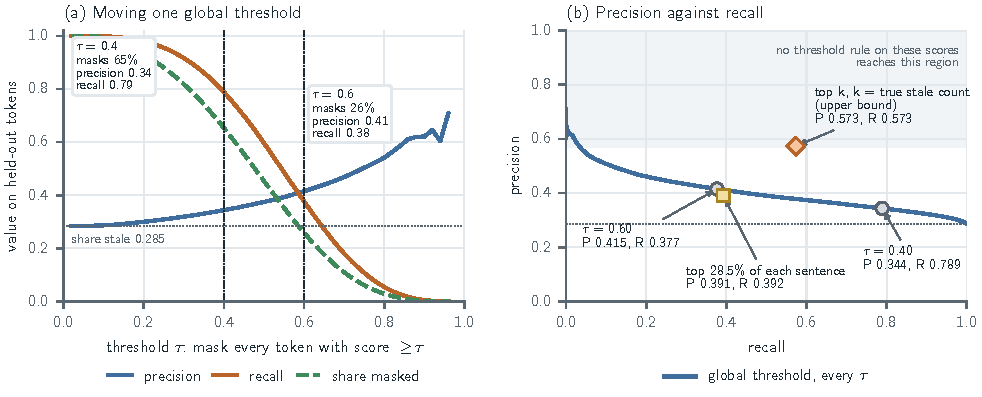
\includegraphics[width=\linewidth]{figures/stale_rules.pdf}
\caption{Masking rules on the held-out tokens. (a)~Precision, recall and masked share as the global threshold $\tau$ varies. Thresholds above 0.96 mask no token and are omitted. (b)~Precision against recall for the global threshold, with the rules of \Cref{tab:rules} marked. The shaded region lies above the upper bound. The dotted line is the share of stale tokens, the precision of random masking.}
\label{fig:stale_rules}
\end{figure}

\begin{figure}[t]
\centering
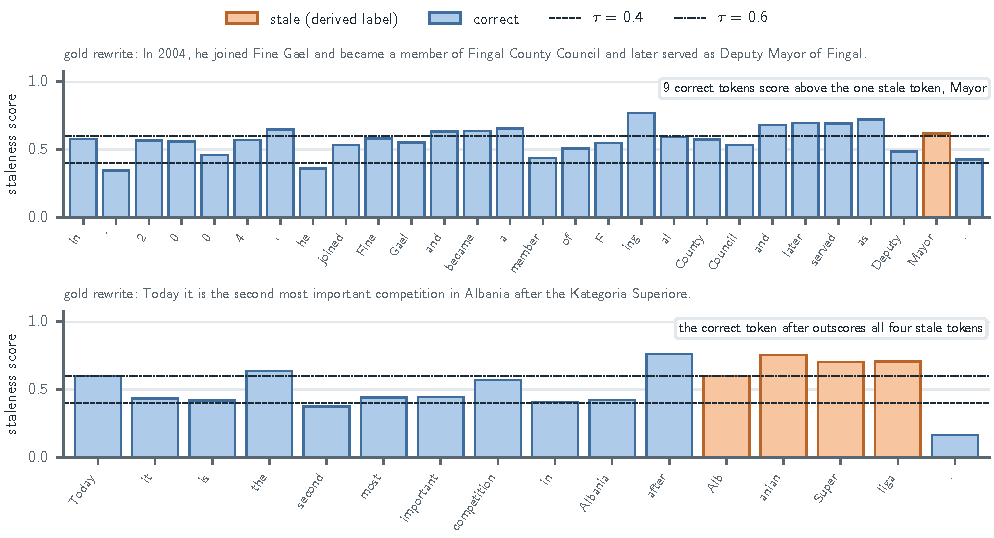
\includegraphics[width=\linewidth]{figures/stale_tokens.pdf}
\caption{Staleness score of each token in two held-out \edit{} sentences. Orange bars are tokens the derived labels mark stale. The gold rewrite appears above each panel. The dashed and dash-dotted lines are the thresholds 0.4 and 0.6.}
\label{fig:stale_tokens}
\end{figure}

\section{Infilling}
\label{sec:infilling}

\subsection{Method}

Each run performs one repair round. Every \drop{} sentence is deleted and every \edit{} sentence is repaired, using the labels derived from the data. Repair has four steps, and Algorithm~\ref{alg:repair} in \Cref{app:code} gives them in full.

\begin{enumerate}
\item \emph{Masks.} The \emph{oracle} setting masks exactly the tokens the derived labels mark stale. The \emph{predicted} setting masks tokens whose staleness score reaches $\tau$, with the fallback, cap and gap rules of Section~7.1 of the design document.
\item \emph{Whole words.} Each masked span widens to the nearest word boundaries. The first run lacked this step. It masked part of the word \emph{hanzi}, kept the remainder \emph{anzi}, and produced \emph{Chinese charactersanzi}.
\item \emph{Candidates.} Spans are filled left to right. Each span is filled at the lengths $\{0, \lceil \ell/2 \rceil, \ell, \ell+2\}$, where $\ell$ is the masked length, with 8 sampler steps.
\item \emph{Reranking.} Each candidate receives the score $0.5 \cdot \text{PLL} + 0.5 \cdot \text{Ent}$ of Eq.~12. PLL, the pseudo-log-likelihood, is the mean log-probability of each token of the sentence with that token masked alone. Ent is the highest probability, over the evidence snippets, that the VitaminC verifier \citep{schuster-etal-2021-vitaminc} assigns to the label ``supports''. The length-zero candidate wins only by a margin of 0.1.
\end{enumerate}

\subsection{Runs}

\Cref{tab:runs} lists the runs. The three \texttt{fix} runs share the same 50 articles, the first 50 of the held-out articles that contain a supported sentence. They repair 106 sentences, 62 of them supported. Within one article of the \texttt{fix-oracle} run, PLL took 1,892 forward passes and the sampler 410, so fluency scoring dominates the cost.

\begin{table}[t]
\caption{Infilling runs. The masked share counts characters of the repaired sentences. In the same sentences, the derived labels mark 22.8\% of characters stale for the \texttt{fix} runs and 26.6\% for \texttt{first}.}
\label{tab:runs}
\centering
\footnotesize
\setlength{\tabcolsep}{4pt}
\begin{tabular}{llccccc}
\toprule
Run & Articles & Masks & Evidence & Whole words & Masked share & Seconds/article \\
\midrule
\texttt{first} & 200 held-out & predicted, $\tau = 0.40$ & yes & no & 55.3\% & 80.8 \\
\texttt{fix-oracle} & 50 supported & oracle & yes & yes & 24.4\% & 49.1 \\
\texttt{fix-oracle-noev} & same 50 & oracle & no & yes & 24.4\% & 13.4 \\
\texttt{fix-predicted} & same 50 & predicted, $\tau = 0.60$ & yes & yes & 33.3\% & 90.9 \\
\bottomrule
\end{tabular}
\end{table}

\subsection{Entity Measures}

\Cref{tab:entities} and \Cref{fig:entities} compare the three \texttt{fix} runs with the unchanged source sentence, which we call \emph{copy}. Copy writes no new entity and keeps every outdated one by construction.

\begin{table}[t]
\caption{Infilling on 106 repaired sentences in 50 articles. Arrows mark the direction of improvement. \emph{Best in pool} is, for each sentence, the oracle-mask candidate with the highest new-entity recall, chosen with the gold rewrite, so it bounds what a better reranker could reach with the same candidates.}
\label{tab:entities}
\centering
\footnotesize
\setlength{\tabcolsep}{4pt}
\begin{tabular}{lcccccc}
\toprule
System & ROUGE-L $\uparrow$ & Precision $\uparrow$ & Recall $\uparrow$ & New-entity & Outdated & Fabricated $\downarrow$ \\
 & & & & recall $\uparrow$ & kept $\downarrow$ & \\
\midrule
Copy (unchanged sentence) & 0.782 & 0.727 & 0.740 & 0.000 & 1.000 & 0.000 \\
Oracle masks & \textbf{0.801} & \textbf{0.753} & \textbf{0.777} & \textbf{0.218} & 0.236 & \textbf{0.144} \\
Oracle masks, no evidence & 0.779 & 0.701 & 0.716 & 0.084 & \textbf{0.197} & 0.229 \\
Predicted masks, $\tau = 0.60$ & 0.678 & 0.578 & 0.587 & 0.134 & 0.472 & 0.247 \\
\midrule
Best in pool, oracle masks & n/a & 0.930 & 0.810 & 0.328 & 0.055 & 0.085 \\
\bottomrule
\end{tabular}
\end{table}

\begin{figure}[t]
\centering
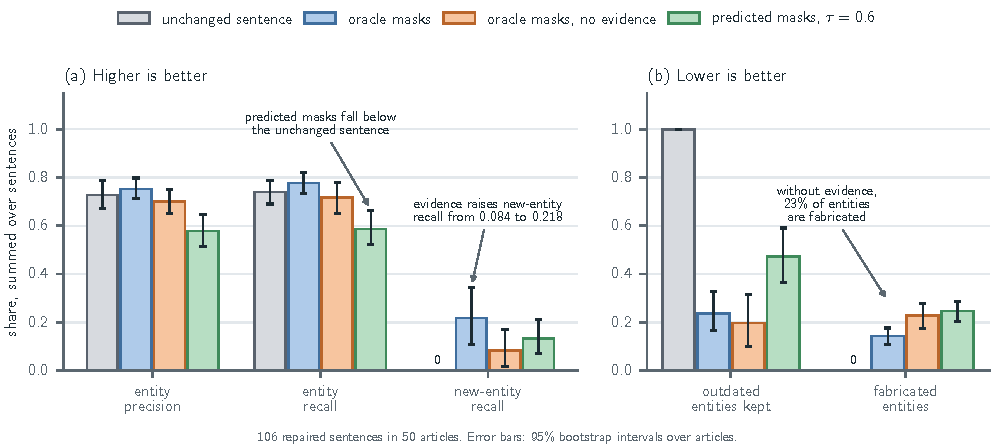
\includegraphics[width=\linewidth]{figures/entities.pdf}
\caption{Entity measures of the four systems on 106 repaired sentences in 50 articles. Error bars are 95\% bootstrap intervals over articles with 10,000 resamples. A 0 marks a bar of height zero.}
\label{fig:entities}
\end{figure}

\paragraph{Oracle masks.} With the true stale tokens masked, the output writes 21.8\% of the entities the update adds and removes 76.4\% of the outdated ones. Its entity precision and recall exceed copy by 0.025 and 0.037, and its ROUGE-L by 0.019. 14.4\% of its entities appear in neither the source nor the evidence.

\paragraph{Evidence.} Without the evidence in the input, new-entity recall falls from 0.218 to 0.084, and fabricated entities rise from 14.4\% to 22.9\%. On the 62 supported sentences, new-entity recall falls from 0.277 to 0.031. The frozen model therefore takes most new entities from the evidence and few from its own memory. This is the check of Risk~1 in the design document, and on these sentences the risk does not occur.

\paragraph{Predicted masks.} With the staleness head's masks at $\tau = 0.60$, entity precision and recall fall about 0.15 below copy, ROUGE-L falls 0.105 below copy, and 47.2\% of outdated entities survive. Widening spans to whole words raises the masked share from 25.8\% of tokens to 33.3\% of characters, against 22.8\% stale.

\paragraph{Reranking.} The candidate pool holds better outputs than the reranker picks. The best candidate per sentence reaches new-entity recall 0.328 and keeps 5.5\% of outdated entities, against 0.218 and 23.6\% for the chosen output. Re-scoring the 1,550 stored decisions of the first run with nine other rules (raw, exponentiated and standardized PLL at weights 0.1 to 0.5, PLL alone, the verifier alone, and a word-overlap score with the evidence) gave mean ROUGE-L between 0.559 and 0.570, against 0.569 for the current rule. The verifier score barely separates candidates. Its median range across the candidates of one decision is 0.002, against 0.374 for PLL, so the chosen candidate equals the most fluent one in 88.5\% of decisions.

\subsection{UpdateROUGE}

\Cref{tab:update_rouge} and \Cref{fig:update_rouge} report UpdateROUGE against two gold sides. The \emph{full} side holds every gold sentence absent from the source, including the sentences the revision added, which the pipeline cannot produce. The \emph{edits} side holds only the gold rewrites of \edit{} sentences, the part of the update the pipeline attempts. The unchanged article scores 0 on both, because it changes no sentence. The first run, on its own 200 articles, scores 0.473 ROUGE-L on the full side and 0.566 on the edits side.

\begin{table}[t]
\caption{UpdateROUGE F1 on the 50 shared articles, mean over articles.}
\label{tab:update_rouge}
\centering
\small
\begin{tabular}{lcccccc}
\toprule
 & \multicolumn{3}{c}{Full gold side} & \multicolumn{3}{c}{Edits gold side} \\
\cmidrule(lr){2-4}\cmidrule(lr){5-7}
System & R-1 & R-2 & R-L & R-1 & R-2 & R-L \\
\midrule
Oracle masks & \textbf{0.668} & \textbf{0.582} & \textbf{0.639} & \textbf{0.750} & \textbf{0.664} & \textbf{0.725} \\
Oracle masks, no evidence & 0.609 & 0.532 & 0.589 & 0.679 & 0.599 & 0.661 \\
Predicted masks, $\tau = 0.60$ & 0.637 & 0.498 & 0.595 & 0.688 & 0.541 & 0.649 \\
\bottomrule
\end{tabular}
\end{table}

\begin{figure}[t]
\centering
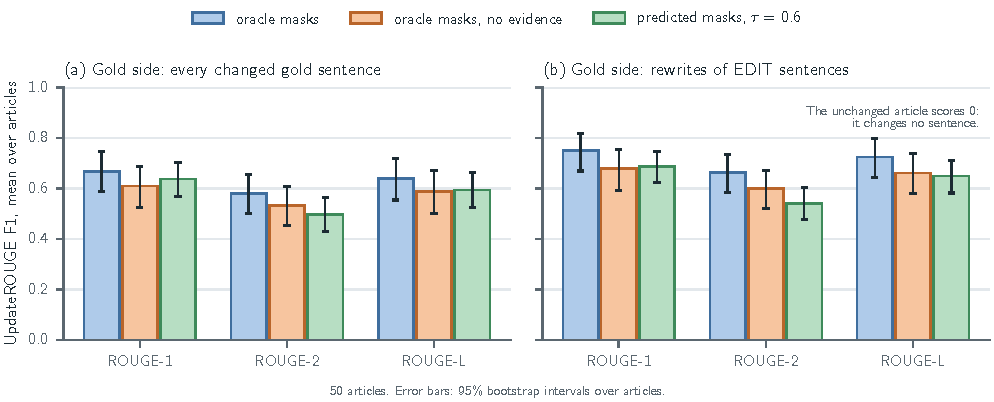
\includegraphics[width=\linewidth]{figures/update_rouge.pdf}
\caption{UpdateROUGE of the three \texttt{fix} runs on 50 articles. (a)~Against every gold sentence absent from the source. (b)~Against the gold rewrites of \edit{} sentences only. Error bars are 95\% bootstrap intervals over articles.}
\label{fig:update_rouge}
\end{figure}

\section{Significance Tests}
\label{sec:tests}

\Cref{fig:differences} and \Cref{tab:tests} report paired tests on the 50 shared articles, with the procedures of \Cref{sec:background}. The Holm correction runs over the 30 tests of the sentence-level table, five pairs of systems on six measures. Comparisons with copy on new-entity recall, outdated kept and fabricated are significant by construction, because copy scores exactly 0, 1 and 0 on them, and \Cref{tab:tests} omits them. UpdateROUGE has its own tables of nine tests per gold side, three pairs on three ROUGE variants.

\begin{figure}[t]
\centering
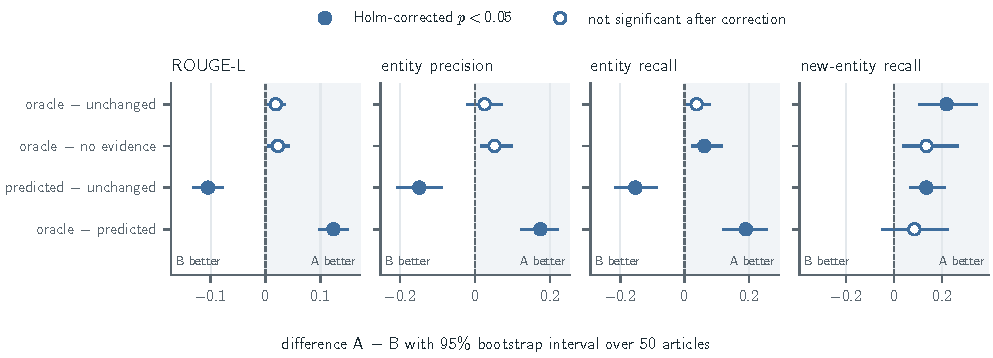
\includegraphics[width=\linewidth]{figures/differences.pdf}
\caption{Paired differences between systems on 106 repaired sentences in 50 articles. Each row is one comparison, A $-$ B. Bars are 95\% bootstrap intervals over articles. Filled markers have a Holm-corrected permutation $p$ below 0.05 over the 30 tests. The oracle-against-unchanged difference in new-entity recall is significant by construction, because the unchanged sentence scores 0.}
\label{fig:differences}
\end{figure}

\begin{table}[t]
\caption{Paired tests on 50 articles. $p$ is the two-sided permutation $p$-value and $p_{\text{Holm}}$ its Holm-corrected value. Bold marks $p_{\text{Holm}} < 0.05$. Sentence-level rows are corrected over 30 tests, UpdateROUGE rows over the nine tests of their gold side.}
\label{tab:tests}
\centering
\footnotesize
\begin{tabular}{llcccc}
\toprule
Comparison (A $-$ B) & Measure & A $-$ B & 95\% interval & $p$ & $p_{\text{Holm}}$ \\
\midrule
Oracle $-$ copy & ROUGE-L & $+0.019$ & $[+0.005, +0.034]$ & 0.010 & 0.093 \\
 & Entity precision & $+0.025$ & $[-0.019, +0.069]$ & 0.306 & 1.000 \\
 & Entity recall & $+0.037$ & $[+0.006, +0.077]$ & 0.052 & 0.417 \\
\midrule
Oracle $-$ no evidence & ROUGE-L & $+0.022$ & $[+0.005, +0.042]$ & 0.009 & 0.091 \\
 & Entity recall & $+0.061$ & $[+0.025, +0.114]$ & $<0.001$ & \textbf{0.005} \\
 & New-entity recall & $+0.134$ & $[+0.038, +0.264]$ & 0.006 & 0.068 \\
 & Fabricated & $-0.085$ & $[-0.121, -0.050]$ & $<0.001$ & \textbf{0.003} \\
 & UpdateROUGE-1, edits & $+0.071$ & $[+0.027, +0.129]$ & $<0.001$ & \textbf{0.006} \\
 & UpdateROUGE-L, edits & $+0.064$ & $[+0.017, +0.122]$ & 0.008 & \textbf{0.0498} \\
\midrule
Predicted $-$ copy & ROUGE-L & $-0.105$ & $[-0.130, -0.078]$ & $<0.001$ & \textbf{0.003} \\
 & Entity precision & $-0.149$ & $[-0.207, -0.091]$ & $<0.001$ & \textbf{0.003} \\
 & Entity recall & $-0.153$ & $[-0.215, -0.089]$ & $<0.001$ & \textbf{0.003} \\
\midrule
Oracle $-$ predicted & ROUGE-L & $+0.124$ & $[+0.098, +0.149]$ & $<0.001$ & \textbf{0.003} \\
 & Entity recall & $+0.190$ & $[+0.121, +0.255]$ & $<0.001$ & \textbf{0.003} \\
 & New-entity recall & $+0.084$ & $[-0.050, +0.223]$ & 0.352 & 1.000 \\
 & Outdated kept & $-0.236$ & $[-0.356, -0.122]$ & 0.002 & \textbf{0.021} \\
 & UpdateROUGE-2, edits & $+0.123$ & $[+0.056, +0.186]$ & $<0.001$ & \textbf{0.004} \\
 & UpdateROUGE-L, edits & $+0.076$ & $[+0.011, +0.135]$ & 0.018 & 0.091 \\
\midrule
No evidence $-$ copy & ROUGE-L & $-0.004$ & $[-0.019, +0.013]$ & 0.717 & 1.000 \\
\bottomrule
\end{tabular}
\end{table}

Three results are significant. Predicted masks make the output worse than copy on ROUGE-L, entity precision and entity recall. Oracle masks beat predicted masks on ROUGE-L, entity recall, outdated entities kept and UpdateROUGE-2. Removing the evidence lowers entity recall and UpdateROUGE on the edits side, and raises fabricated entities.

Two results are not significant after the correction. Oracle masks beat copy on ROUGE-L by 0.019, an interval that excludes zero and an uncorrected $p$ of 0.010, but the corrected $p$ is 0.093. The gain in new-entity recall from the evidence, 0.134, has corrected $p$ 0.068.

The sentence-level correction covers 9 comparisons with copy that are significant by construction, so it is stricter than a correction over the informative tests alone. The uncorrected $p$-values are in \texttt{runs/significance.json} and \texttt{runs/update\_rouge.json}.

\section{Examples}
\label{sec:examples}

The examples below come from the training data and from the saved infilling runs, and a script copies every sentence from those files by article and sentence index. Each example names its article. The data examples D1 to D9 show the ways a derived label can be wrong. The infilling examples I1 to I8 show what the frozen model writes under oracle masks, without the evidence, and under the staleness head's masks, all taken from the same sentence of the three \texttt{fix} runs unless stated.

% generated by analysis/report_examples.py, do not edit by hand

\subsection{Data}

\begin{table}[H]
\footnotesize
\begin{tabular}{@{}p{0.17\linewidth}p{0.79\linewidth}@{}}
\toprule
\multicolumn{2}{@{}l}{\textbf{D1. An edit whose new numbers the evidence does not contain (train-000004, sentence 2)}} \\
\midrule
\textsf{Source} & He played 321 games for the club, scoring 37 goals. \\
\textsf{Gold rewrite} & He played 327 matches for the club, scoring 38 goals. \\
\textsf{Label} & \edit{} (similarity 0.75) \\
\midrule
\multicolumn{2}{@{}p{0.97\linewidth}@{}}{The revision updated the career totals, but no snippet of the article's evidence, cut or uncut, contains 327 or 38. No system can derive this rewrite from its input, yet the label asks for it. Only 16.9\% of edited sentences with new words have those words in the input.} \\
\bottomrule
\end{tabular}
\end{table}

\begin{table}[H]
\footnotesize
\begin{tabular}{@{}p{0.17\linewidth}p{0.79\linewidth}@{}}
\toprule
\multicolumn{2}{@{}l}{\textbf{D2. A source sentence paired with an unrelated target fragment (train-000004, sentence 4)}} \\
\midrule
\textsf{Source} & FC Lokomotive was renamed to VfB Leipzig. \\
\textsf{Paired target} & FC Lokomotive Leipzig 39:20. \\
\textsf{Label} & \edit{} (similarity 0.53) \\
\midrule
\multicolumn{2}{@{}p{0.97\linewidth}@{}}{The target sentence is a fragment of a linearized results table. It shares the words FC, Lokomotive and Leipzig with the source, which puts the similarity at 0.53, above the 0.35 floor. The aligner pairs the two and the diff marks ``was renamed to VfB Leipzig'' stale.} \\
\bottomrule
\end{tabular}
\end{table}

\begin{table}[H]
\footnotesize
\begin{tabular}{@{}p{0.17\linewidth}p{0.79\linewidth}@{}}
\toprule
\multicolumn{2}{@{}l}{\textbf{D3. Two source sentences merged into one target sentence (train-000159, sentences 2 and 3)}} \\
\midrule
\textsf{Source 2} & Users of Nextdoor submit their real names and addresses (or street without the exact number) to the website. \\
\textsf{Source 3} & Posts made to the website are available only to other Nextdoor members living in the same neighborhood. \\
\textsf{Target} & Users of Nextdoor are required to submit their real names and addresses (or street without the exact number) to the website; posts made to the website are available only to other Nextdoor members living in the same neighborhood. \\
\textsf{Labels} & source 2: \edit{} (similarity 0.67); source 3: \drop{}, its best similarity 0.60 is to the same target \\
\midrule
\multicolumn{2}{@{}p{0.97\linewidth}@{}}{The revision joined the two sentences with a semicolon. Each target sentence can pair with one source sentence, so source 2 takes the merged sentence first (0.67) and source 3, whose content survives unchanged, becomes \drop{}.} \\
\bottomrule
\end{tabular}
\end{table}

\begin{table}[H]
\footnotesize
\begin{tabular}{@{}p{0.17\linewidth}p{0.79\linewidth}@{}}
\toprule
\multicolumn{2}{@{}l}{\textbf{D4. A sentence split inside a quoted title (train-000780, sentence 3)}} \\
\midrule
\textsf{Source 3} & He contributes a column called "{[}Making{]} No Bones About It{[}! \\
\textsf{Source 4} & {]}", which features on the inside back cover of the weekly \textquotesingle\textquotesingle{}Donegal News\textquotesingle\textquotesingle{}. \\
\textsf{Label of source 3} & \drop{} \\
\midrule
\multicolumn{2}{@{}p{0.97\linewidth}@{}}{spaCy split the sentence at the exclamation mark inside the column's name. The second half pairs with the rewritten target, and the first half becomes \drop{}. The hand review found 6 such non-sentences among 117 flagged rows, including a lone full stop, ``(image)'' and ``\_\_TOC\_\_''.} \\
\bottomrule
\end{tabular}
\end{table}

\begin{table}[H]
\footnotesize
\begin{tabular}{@{}p{0.17\linewidth}p{0.79\linewidth}@{}}
\toprule
\multicolumn{2}{@{}l}{\textbf{D5. The KEEP fix turns a reformatted date into an edit (train-000003, sentence 0)}} \\
\midrule
\textsf{Source} & Jo Jung-suk (born 26 December 1980) is a South Korean actor. \\
\textsf{Gold rewrite} & Jo Jung-suk (born December 26, 1980) is a South Korean actor. \\
\textsf{Label} & before the fix \keep{}, after the fix \edit{} (similarity 0.97) \\
\midrule
\multicolumn{2}{@{}p{0.97\linewidth}@{}}{The date only changed format, but 26 and 1980 contain digits, so the \keep{} fix labels the sentence \edit{} and marks the date stale. A diacritic added to Bhagavad Gita in train-000012 becomes an \edit{} the same way. The fix exists for cases like D6.} \\
\bottomrule
\end{tabular}
\end{table}

\begin{table}[H]
\footnotesize
\begin{tabular}{@{}p{0.17\linewidth}p{0.79\linewidth}@{}}
\toprule
\multicolumn{2}{@{}l}{\textbf{D6. A real update the fix catches (train-057216, sentence 0, from the hand review)}} \\
\midrule
\textsf{Source} & David Turnbull (born 10 July 1999) is a Scottish professional footballer who plays as a midfielder for Motherwell. \\
\textsf{Gold rewrite} & David Turnbull (born 10 July 1999) is a Scottish professional footballer who plays as a midfielder for Celtic. \\
\textsf{Label} & before the fix \keep{}, after the fix \edit{} (similarity 0.95) \\
\midrule
\multicolumn{2}{@{}p{0.97\linewidth}@{}}{A one-word club change keeps the similarity above 0.95, so the first build labelled the sentence \keep{}. The reviewer marked it \edit{}, as for 8 of the 24 errors found, and the fix now agrees.} \\
\bottomrule
\end{tabular}
\end{table}

\begin{table}[H]
\footnotesize
\begin{tabular}{@{}p{0.17\linewidth}p{0.79\linewidth}@{}}
\toprule
\multicolumn{2}{@{}l}{\textbf{D7. A rephrasing labelled as an edit (train-042079, sentence 0, from the hand review)}} \\
\midrule
\textsf{Source} & The Chicago Bulls are an American professional basketball team based in Chicago, Illinois. \\
\textsf{Gold rewrite} & The Chicago Bulls are an American professional basketball team based in Chicago. \\
\textsf{Label} & \edit{} (similarity 0.93) \\
\midrule
\multicolumn{2}{@{}p{0.97\linewidth}@{}}{The revision dropped the state name without changing any fact. The reviewer judged the label wrong and the sentence \keep{}, as for 13 of the 24 errors found. The staleness head still learns to treat ``Illinois'' as stale.} \\
\bottomrule
\end{tabular}
\end{table}

\begin{table}[H]
\footnotesize
\begin{tabular}{@{}p{0.17\linewidth}p{0.79\linewidth}@{}}
\toprule
\multicolumn{2}{@{}l}{\textbf{D8. The evidence that supports an update cut by the token budget (train-000862, sentence 5)}} \\
\midrule
\textsf{Source} & The current Chief Justice is the Hon'ble Justice Mohammad Rafiq who took oath as Chief Justice on 13 November 2019. \\
\textsf{Gold rewrite} & The current Chief Justice is the Hon'ble Justice Biswanath Somadder who took oath on 27 April 2020. \\
\textsf{Evidence} & The snippet titled ``Biswanath Somadder'' kept 0 of its 118 characters after the cut. \\
\midrule
\multicolumn{2}{@{}p{0.97\linewidth}@{}}{The snippets are ordered by how many mentions they share with the old article. The snippet about the new Chief Justice shares none, so it comes last and the 600-token budget empties it. The input then lacks the name and the date the update needs.} \\
\bottomrule
\end{tabular}
\end{table}

\begin{table}[H]
\footnotesize
\begin{tabular}{@{}p{0.17\linewidth}p{0.79\linewidth}@{}}
\toprule
\multicolumn{2}{@{}l}{\textbf{D9. A stylistic change marked stale (train-002320, sentence 0)}} \\
\midrule
\textsf{Source} & The Appian Way Regional Park is a protected area of around 3400 hectares, established by the Italian region of Latium. \\
\textsf{Gold rewrite} & It is a protected area of around 4580 hectares, established by the Italian region of Latium. \\
\textsf{Stale spans} & ``The Appian Way Regional Park'', ``3400'' \\
\midrule
\multicolumn{2}{@{}p{0.97\linewidth}@{}}{The diff marks both the new area and the replacement of the park's name by ``It''. Only the first is a fact the evidence states. The second is a style choice of the revision.} \\
\bottomrule
\end{tabular}
\end{table}

\subsection{Infilling}

\begin{table}[H]
\footnotesize
\begin{tabular}{@{}p{0.17\linewidth}p{0.79\linewidth}@{}}
\toprule
\multicolumn{2}{@{}l}{\textbf{I1. The evidence supplies the new club (train-000184, sentence 0)}} \\
\midrule
\textsf{Source} & Simone Corazza (born 22 March 1991) is an Italian footballer who currently plays for Reggina. \\
\textsf{Oracle masks} & ``Reggina'' \\
\textsf{Gold rewrite} & Simone Corazza (born 22 March 1991) is an Italian footballer who currently plays for Alessandria. \\
\textsf{Oracle output} & Simone Corazza (born 22 March 1991) is an Italian footballer who currently plays for Italian club Alessandria. \\
\textsf{No evidence} & Simone Corazza (born 22 March 1991) is an Italian footballer who currently plays for Serie B club Cesena. \\
\textsf{Predicted masks} & Simone Corazza (born 22 March 1991) is an Italian footballer who currently plays for Italian club Alessandria. \\
\midrule
\multicolumn{2}{@{}p{0.97\linewidth}@{}}{With the evidence, the model writes the right club. Without it, the model writes a plausible but wrong club and league. The entity measures count ``Alessandria'' as fabricated, because the evidence names the club only inside a linearized table, where spaCy finds no entities. Counting a mention as supported when its text occurs in the evidence lowers the fabricated share of the oracle run from 14.4\% to 10.6\%, of the run without evidence from 22.9\% to 19.9\%, and of the predicted run from 24.7\% to 18.7\%.} \\
\bottomrule
\end{tabular}
\end{table}

\begin{table}[H]
\footnotesize
\begin{tabular}{@{}p{0.17\linewidth}p{0.79\linewidth}@{}}
\toprule
\multicolumn{2}{@{}l}{\textbf{I2. A transfer the model reads from the evidence (train-001621, sentence 0)}} \\
\midrule
\textsf{Source} & Brian Oliván Herrero (born 1 April 1994) is a Spanish professional footballer who plays for Girona FC on loan from Cádiz CF as a left back. \\
\textsf{Oracle masks} & ``Girona FC on loan from Cádiz CF'' \\
\textsf{Gold rewrite} & Brian Oliván Herrero (born 1 April 1994) is a Spanish professional footballer who plays for RCD Mallorca as a left back. \\
\textsf{Oracle output} & Brian Oliván Herrero (born 1 April 1994) is a Spanish professional footballer who plays for RCD Mallorca on loan from Cádiz CF as a left back. \\
\textsf{No evidence} & Brian Oliván Herrero (born 1 April 1994) is a Spanish professional footballer who plays for CD Tenerife, on loan from Real Betis, as a left back. \\
\midrule
\multicolumn{2}{@{}p{0.97\linewidth}@{}}{The oracle output takes RCD Mallorca from the evidence but keeps ``on loan from Cádiz CF'', because the mask set covers it and the chosen candidate refilled it. Without the evidence, the model invents a different club and a different loan.} \\
\bottomrule
\end{tabular}
\end{table}

\begin{table}[H]
\footnotesize
\begin{tabular}{@{}p{0.17\linewidth}p{0.79\linewidth}@{}}
\toprule
\multicolumn{2}{@{}l}{\textbf{I3. A number the model cannot recover (train-002079, sentence 1)}} \\
\midrule
\textsf{Source} & It has a population of 7,541 people (Canada 2011 Census). \\
\textsf{Oracle masks} & ``It'', ``541'', ``Canada 2011'' \\
\textsf{Gold rewrite} & Located on Lake Gilman it has a population of 7,504 people (2016 Canadian Census). \\
\textsf{Oracle output} & It has a population of 7,000 Cree people (Canada 2006 Census). \\
\textsf{Predicted masks} & It has a population of 800 and an area of  (Canada 2006). The town of \\
\midrule
\multicolumn{2}{@{}p{0.97\linewidth}@{}}{The word diff splits 7,541 at the comma, so only 541 is stale. The model fills it with a round 000, adds ``Cree'', and writes 2006 for the census year. The predicted masks cover the number and the census, and the output breaks off mid-sentence.} \\
\bottomrule
\end{tabular}
\end{table}

\begin{table}[H]
\footnotesize
\begin{tabular}{@{}p{0.17\linewidth}p{0.79\linewidth}@{}}
\toprule
\multicolumn{2}{@{}l}{\textbf{I4. Oracle masks too small to express the rewrite (train-000076, sentence 0)}} \\
\midrule
\textsf{Source} & Monterrey is a district in Aserrí Canton, Costa Rica. \\
\textsf{Oracle masks} & ``in'', ``,'' \\
\textsf{Gold rewrite} & Monterrey is a district of the Aserrí canton, in the San José province of Costa Rica. \\
\textsf{Oracle output} & Monterrey is a district in Aserrí Canton, Costa Rica. \\
\textsf{Predicted masks} & Monterrey is a district in the San José province of Costa Rica. \\
\midrule
\multicolumn{2}{@{}p{0.97\linewidth}@{}}{The diff marks only ``in'' and the comma, the anchors of two insertions. Lengths up to the masked length plus two cannot hold ``the San José province of'', so the oracle run returns the source unchanged. The predicted mask covers ``Aserrí Canton, Costa Rica'', and the output names the province but drops the canton.} \\
\bottomrule
\end{tabular}
\end{table}

\begin{table}[H]
\footnotesize
\begin{tabular}{@{}p{0.17\linewidth}p{0.79\linewidth}@{}}
\toprule
\multicolumn{2}{@{}l}{\textbf{I5. Predicted masks rewrite correct text (train-001500, sentence 2)}} \\
\midrule
\textsf{Source} & KFFX's studios are located on Clearwater Avenue in Kennewick, and its transmitter is located in the Umatilla National Forest east of Pendleton. \\
\textsf{Gold rewrite} & KFFX-TV's studios are located on Clearwater Avenue in Kennewick, and its transmitter is located in the Umatilla National Forest east of Pendleton. \\
\textsf{Oracle output} & The station's studios are located on Clearwater Avenue in Kennewick, and its transmitter is located in the Umatilla National Forest east of Pendleton. \\
\textsf{Predicted masks} & The station's studios are located on Clearwater Avenue in Kennewick, and its transmitter and tower are located in the Umatilla National Forest east of Richland. \\
\midrule
\multicolumn{2}{@{}p{0.97\linewidth}@{}}{The update only renames the station. The predicted masks also cover ``is'' and ``Pendleton'', and the model replaces the correct Pendleton with Richland.} \\
\bottomrule
\end{tabular}
\end{table}

\begin{table}[H]
\footnotesize
\begin{tabular}{@{}p{0.17\linewidth}p{0.79\linewidth}@{}}
\toprule
\multicolumn{2}{@{}l}{\textbf{I6. A typo repaired, and a new error introduced (train-000455, sentence 2)}} \\
\midrule
\textsf{Source} & Brag previously served as the operations director of Operation Inherent Resolve, the official name for US war on ISIS. \\
\textsf{Gold rewrite} & Braga previously served as the operations director of Operation Inherent Resolve, the official name for US war on ISIS. \\
\textsf{Oracle output} & Braga previously served as the operations director of Operation Inherent Resolve, the official name for US war on ISIS. \\
\textsf{No evidence} & He has previously served as the operations director of Operation Inherent Resolve, the official name for US war on ISIS. \\
\textsf{Predicted masks} & He has previously served as the operations director of Operation Inherent Resolve, the official name of the United States mission in Afghanistan. \\
\midrule
\multicolumn{2}{@{}p{0.97\linewidth}@{}}{The oracle output fixes the misspelled name. The predicted masks also cover ``name for US war on ISIS'', and the model turns the war on ISIS into a mission in Afghanistan.} \\
\bottomrule
\end{tabular}
\end{table}

\begin{table}[H]
\footnotesize
\begin{tabular}{@{}p{0.17\linewidth}p{0.79\linewidth}@{}}
\toprule
\multicolumn{2}{@{}l}{\textbf{I7. A list item updated from the evidence (train-000101, sentence 4)}} \\
\midrule
\textsf{Source} & (1991), \textquotesingle\textquotesingle{}Freddy Got Fingered\textquotesingle\textquotesingle{} (2001), \textquotesingle\textquotesingle{}A Master Builder\textquotesingle\textquotesingle{} (2014) and \textquotesingle\textquotesingle{}Instant Family\textquotesingle\textquotesingle{} (2018). \\
\textsf{Gold rewrite} & (1991), \textquotesingle\textquotesingle{}Freddy Got Fingered\textquotesingle\textquotesingle{} (2001), \textquotesingle\textquotesingle{}A Master Builder\textquotesingle\textquotesingle{} (2014), and \textquotesingle\textquotesingle{}Marriage Story\textquotesingle\textquotesingle{} (2019). \\
\textsf{Oracle output} & (1991), \textquotesingle\textquotesingle{}Freddy Got Fingered\textquotesingle\textquotesingle{} (2001), \textquotesingle\textquotesingle{}A Master Builder\textquotesingle\textquotesingle{} (2014), and \textquotesingle\textquotesingle{}Marriage Story\textquotesingle\textquotesingle{} (both 2019). \\
\textsf{No evidence} & (1991), \textquotesingle\textquotesingle{}Freddy Got Fingered\textquotesingle\textquotesingle{} (2001), \textquotesingle\textquotesingle{}A Master Builder\textquotesingle\textquotesingle{} (2014), and \textquotesingle\textquotesingle{}The Book of Life\textquotesingle\textquotesingle{} (2017–present). \\
\textsf{Predicted masks} & (1991), \textquotesingle\textquotesingle{}Freddy Got Fingered\textquotesingle\textquotesingle{} (2001), the documentary \textquotesingle\textquotesingle{}A Master Builder\textquotesingle\textquotesingle{} (uncredited), \textquotesingle\textquotesingle{}Instant Karma\textquotesingle\textquotesingle{} (200 \\
\midrule
\multicolumn{2}{@{}p{0.97\linewidth}@{}}{With the evidence, the model writes the new film and year, with a spurious ``both''. Without it, the model invents a different title and year range.} \\
\bottomrule
\end{tabular}
\end{table}

\begin{table}[H]
\footnotesize
\begin{tabular}{@{}p{0.17\linewidth}p{0.79\linewidth}@{}}
\toprule
\multicolumn{2}{@{}l}{\textbf{I8. A mask that cut a word in half, first run (train-000000, sentence 1)}} \\
\midrule
\textsf{Source} & Chinese characters (including Chinese hanzi, Japanese kanji and Korean hanja) are logograms; some Egyptian hieroglyphs and some graphemes in cuneiform script are also logograms. \\
\textsf{Masked spans} & ``(including Chinese h'', ``kanji and Korean hanja) are logograms;'', ``s'', ``graphemes in c'', ``script are also logograms'' \\
\textsf{A candidate} & Chinese charactersanzi, Japanese kanji, Korean hanja, Chinese numerals, some Egyptian hieroglyphs and some Mesopotamian cuneiform signs are all logograms. \\
\midrule
\multicolumn{2}{@{}p{0.97\linewidth}@{}}{The token mask covered ``h'' of ``hanzi'' but not the rest of the word. The length-zero candidate then joined ``characters'' and ``anzi''. Widening masks to whole words removes this failure.} \\
\bottomrule
\end{tabular}
\end{table}


\section{Findings and Next Steps}
\label{sec:findings}

\subsection{Findings}

\begin{enumerate}
\item The label noise is lower than the earlier documents state. The 40 to 60\% figure is a confident-learning estimate from a classifier with macro-F1 0.506. A hand review of the 111 sentences that estimate disputes most found 21.6\% wrong.
\item Only 16.9\% of edited sentences with new words have those words in the input, which bounds how much any system can recover on the silver data.
\item LLaDA states beat a sentence encoder without LLaDA by 0.064 macro-F1 for sentence labels, averaged over five seeds, a significant difference. Focal loss lowers macro-F1 by about 0.009 and staleness AUROC by 0.019, and no evidence feature tested raises macro-F1. Results vary little across seeds, with standard deviations of 0.003 or less.
\item The staleness head limits the system. Its AUROC is 0.645, no threshold rule exceeds precision 0.573, and its masks make the output significantly worse than the unchanged sentence.
\item With correct masks and the evidence in the input, the frozen model writes new entities from the evidence. Removing the evidence significantly raises fabricated entities and lowers entity recall and UpdateROUGE.
\item With correct masks, the gain over the unchanged sentence (0.019 ROUGE-L, 0.037 entity recall) is not significant on 50 articles.
\item The candidate pool contains outputs with 0.110 more new-entity recall than the reranker picks. The verifier term varies too little between candidates to change the ranking.
\end{enumerate}

\subsection{Limitations}

All labels are silver, and the random-sample audit that would measure their noise has not been reviewed. All numbers come from held-out training articles, not from the validation split or the gold test set. The infilling runs use derived sentence labels, one round and 50 articles, so their intervals are wide. At the measured 49.1 seconds per article, 200 articles would take about 2.7 hours of GPU time per oracle run and would roughly halve the interval widths.

\subsection{Next Steps}

\begin{enumerate}
\item \emph{Label audit.} Review the 436 sentences of \texttt{audit/train\_audit.tsv} to measure the noise rate on a random sample, with a second reviewer on a shared subset for agreement.
\item \emph{Staleness head.} Add per-token evidence features, such as whether the token's word appears in the evidence and the similarity to the nearest snippet. Replace the linear layer with a small MLP over the token state, the sentence vector and the nearest-snippet vector. Train only on supported edits. All three use the stored features and need no new LLaDA pass.
\item \emph{Reranker.} Add a term that raises the score of a candidate for each evidence entity it contains and lowers it for each source entity absent from the evidence, and test it first on the stored candidates.
\item \emph{Cascade through the evidence.} Replace the trained cascade detector with a simpler loop. After each round, append the rewritten sentences to the evidence of the next round, then run the classifier and the staleness head again on the whole article. A sentence that a repair made wrong now conflicts with a sentence in the evidence, so the same heads that find directly contradicted sentences may also find cascades, with no consequence head and no pair mining. Cascade recall on the hand-labelled cascade set of Section~8.5 of the design document would measure whether this works.
\item \emph{Remaining design.} Build the loop over rounds and the connection from the classifier to infilling, then evaluate on the validation split.
\end{enumerate}

\clearpage
\bibliographystyle{plainnat}
\bibliography{../paper/paper,progress}

\clearpage
\setlength{\intextsep}{8pt plus 2pt minus 2pt}
\beginappendix{}

\section{Code and Algorithms}
\label{app:code}

\Cref{tab:modules} maps each step to its module. Every path starts in \texttt{code/}. Algorithms~\ref{alg:align} to~\ref{alg:tests} give the procedures, with the constants the runs used.

\begin{table}[H]
\caption{Modules of the data build and the pipeline. Every path starts in \texttt{code/}.}
\label{tab:modules}
\footnotesize
\begin{tabular*}{\linewidth}{@{}l@{\extracolsep{\fill}}l@{}}
\toprule
Module & What it does \\
\midrule
\texttt{datasets/fruit/load.py} & Reads FRUIT TFRecords and their markers \\
\texttt{datasets/collate.py} & Builds the splits, the aligner and the labels \\
\texttt{datasets/audit/review.py} & Terminal tool for the label audit \\
\texttt{pipeline/classifier/inputs.py} & Builds the LLaDA input and its sentence spans \\
\texttt{pipeline/classifier/extract.py} & One forward pass per article, stores hidden states \\
\texttt{pipeline/classifier/train.py} & Sentence head, cross-entropy or focal loss \\
\texttt{pipeline/experiments/evidence\_train.py} & Sentence head with an evidence vector \\
\texttt{pipeline/experiments/baseline\_train.py} & The same head on MiniLM embeddings \\
\texttt{pipeline/staleness/train.py} & Token head, binary cross-entropy or focal loss \\
\texttt{pipeline/staleness/sweep.py} & Precision, recall and masked share per threshold \\
\texttt{pipeline/infilling/spans.py} & Masking policy, whole-word widening, lengths \\
\texttt{pipeline/infilling/sampler.py} & LLaDA infilling with low-confidence remasking \\
\texttt{pipeline/infilling/model.py} & Frozen LLaDA wrapper with logits at chosen positions \\
\texttt{pipeline/infilling/score.py} & PLL, the VitaminC verifier and candidate selection \\
\texttt{pipeline/infilling/repair.py} & Repair of one \edit{} sentence \\
\texttt{pipeline/infilling/run.py} & One repair round over a set of articles \\
\texttt{pipeline/infilling/evaluate.py} & ROUGE, hit and coverage \\
\texttt{pipeline/infilling/entities.py} & Entity measures \\
\texttt{pipeline/infilling/update\_rouge.py} & UpdateROUGE with paired tests \\
\texttt{pipeline/infilling/significance.py} & Paired bootstrap, permutation test and Holm correction \\
\texttt{pipeline/analysis/classifier\_tests.py} & Paired tests between sentence classifiers \\
\texttt{pipeline/analysis/stale\_analysis.py} & Threshold rules and examples of the staleness head \\
\texttt{pipeline/analysis/stale\_scatter.py} & Score bins and the 2-D view of token states \\
\texttt{pipeline/analysis/progress\_figures.py} & The figures of this report \\
\texttt{pipeline/analysis/report\_examples.py} & The example tables of \Cref{sec:examples} \\
\bottomrule
\end{tabular*}
\end{table}

\begin{algorithm}[H]
\caption{Sentence alignment and labels (\texttt{collate.label\_sentences}).}
\label{alg:align}
\begin{algorithmic}[1]
\Require source sentences $s_1, \dots, s_n$, target sentences $t_1, \dots, t_m$
\State tokenize each sentence into lowercase words and punctuation marks
\State $P \gets$ all pairs $(i, j)$ with similarity $\text{sim}(s_i, t_j)$, the F1 of the token multisets
\State sort $P$ by similarity descending, then $|i - j|$ ascending, then $i$ ascending
\State $\text{pair} \gets \{\}$
\For{$(i, j) \in P$}
  \If{$\text{sim}(s_i, t_j) < 0.35$} \textbf{break} \EndIf
  \If{$s_i$ and $t_j$ are both unpaired} $\text{pair}[i] \gets j$ \EndIf
\EndFor
\For{$i = 1, \dots, n$}
  \If{$i$ is unpaired} label $s_i$ \drop{}
  \ElsIf{$\text{sim}(s_i, t_{\text{pair}[i]}) \ge 0.95$ and no changed word contains a capital or a digit} label $s_i$ \keep{}
  \Else{} label $s_i$ \edit{} and derive its stale spans (Algorithm~\ref{alg:stale})
  \EndIf
\EndFor
\State every unpaired $t_j$ is an addition
\end{algorithmic}
\end{algorithm}

\begin{algorithm}[H]
\caption{Stale spans of an \edit{} sentence (\texttt{collate.edit\_fields}).}
\label{alg:stale}
\begin{algorithmic}[1]
\Require source tokens $a_1, \dots, a_p$, partner tokens $b_1, \dots, b_q$, lowercased
\State $\text{ops} \gets$ the opcodes of \texttt{difflib.SequenceMatcher}$(a, b)$, without the junk heuristic
\State $\text{stale} \gets \{\}$
\For{each operation on source range $[i_1, i_2)$}
  \If{replace or delete} add $i_1, \dots, i_2 - 1$ to stale \EndIf
  \If{insert} add $i_1 - 1$ to stale, or token 0 at the start of the sentence \EndIf
\EndFor
\State merge consecutive stale tokens into character spans of the source sentence
\end{algorithmic}
\end{algorithm}

\begin{algorithm}[H]
\caption{Confident-learning estimate of label noise, as reported in \texttt{audit/noise.json}.}
\label{alg:cl}
\begin{algorithmic}[1]
\Require out-of-fold class probabilities $\hat{p}_j$ and given labels $y_j$ for every sentence $j$
\For{each class $c$} $t_c \gets$ mean of $\hat{p}_{j,c}$ over sentences with $y_j = c$ \EndFor
\For{each sentence $j$}
  \State $A \gets \{c : \hat{p}_{j,c} \ge t_c\}$
  \If{$A$ is not empty} $C[y_j][\arg\max_{c \in A} \hat{p}_{j,c}] \mathrel{+}= 1$ \EndIf
\EndFor
\State rescale each row of $C$ so that it sums to the number of sentences with that given label
\For{each class $c$} noise rate of $c$ $\gets$ off-diagonal sum of row $c$ / row sum \EndFor
\end{algorithmic}
\end{algorithm}

\begin{algorithm}[H]
\caption{Repair of one \edit{} sentence (\texttt{spans.policy\_spans}, \texttt{spans.snap}, \texttt{repair.repair\_sentence}).}
\label{alg:repair}
\begin{algorithmic}[1]
\Require token staleness scores $\pi_i$ or derived stale tokens, threshold $\tau$
\State mask tokens with $\pi_i \ge \tau$, or the top fifth if none reach it, at most half the sentence
\State fill single-token gaps between masked tokens
\State widen each masked span to word boundaries and merge spans that touch
\For{each span, left to right}
  \For{each length $n \in \{0, \lceil \ell/2 \rceil, \ell, \ell + 2\}$}
    \State put $n$ masks at the span, keep later spans at their own length, add the full context
    \State fill the masks over 8 steps, committing the most confident predictions first
    \State $\text{PLL} \gets$ mean log-probability of each sentence token, masked one at a time
    \State $\text{Ent} \gets$ highest VitaminC support probability over the evidence snippets
    \State score $\gets 0.5 \cdot \text{PLL} + 0.5 \cdot \text{Ent}$
  \EndFor
  \State keep the best candidate, where the length-0 candidate needs a margin of 0.1
\EndFor
\end{algorithmic}
\end{algorithm}

\begin{algorithm}[H]
\caption{Paired tests over articles (\texttt{significance.test}, \texttt{significance.holm}).}
\label{alg:tests}
\begin{algorithmic}[1]
\Require per article $a$, summed numerators and denominators $(n^A_a, d^A_a)$ and $(n^B_a, d^B_a)$ of a measure
\State $\Delta \gets \sum_a n^A_a / \sum_a d^A_a - \sum_a n^B_a / \sum_a d^B_a$
\For{$r = 1, \dots, 10{,}000$}
  \State draw articles with replacement and recompute $\Delta$ on them \Comment{bootstrap}
  \State swap A and B inside each article with probability $\tfrac12$ and recompute $\Delta$ \Comment{permutation}
\EndFor
\State interval $\gets$ 2.5th and 97.5th percentiles of the bootstrap values
\State $p \gets (1 + \#\{|\Delta_{\text{perm}}| \ge |\Delta|\}) / 10{,}001$
\State Holm: sort the $m$ $p$-values ascending, multiply the $k$-th by $m - k + 1$, take running maxima, cap at 1
\end{algorithmic}
\end{algorithm}

\end{document}
